\documentclass[11pt,a4paper]{article}
\usepackage[T1]{fontenc}
\usepackage[utf8]{inputenc}
\usepackage[french]{babel}
\usepackage{amsmath,amssymb,booktabs,longtable,array}
\usepackage[a4paper,margin=2.25cm]{geometry}
\usepackage{graphicx}
\usepackage[hidelinks]{hyperref}
\usepackage{microtype}
\usepackage{enumitem}
\usepackage{titlesec}
\usepackage{tcolorbox}
\tcbuselibrary{skins,breakable}

\setlength{\parindent}{0pt}
\setlength{\parskip}{0.5em}
\titleformat{\section}{\large\bfseries}{\thesection}{0.6em}{}
\titleformat{\subsection}{\normalsize\bfseries}{\thesubsection}{0.6em}{}

\newtcolorbox{verdictbox}{
  breakable, enhanced, colback=black!3, colframe=black!55,
  boxrule=0.4pt, arc=1pt, left=8pt, right=8pt, top=6pt, bottom=6pt
}

\title{Synthèse finale — réplication critique de M2\\
\large Distribution Boltzmann--Pareto par auto-organisation critique : bilan}
\author{Réplication computationnelle indépendante}
\date{3 juillet 2026}

\begin{document}
\maketitle

\begin{verdictbox}
\textbf{Verdict exécutif.} M2 a été implémenté et testé, mais la thèse
« distribution Boltzmann--Pareto émergente par auto-organisation critique »
n'est pas confirmée. Le modèle produit des classes fortement renouvelées et un
régime démographique de taille finie sur la baseline. Il ne produit pas de
corps exponentiel. Sa queue est compatible avec une pente de type Pareto sur
une plage limitée, mais une log-normale tronquée a une meilleure vraisemblance
dans toutes les comparaisons. La même queue apparente subsiste sans crédit, ce
qui réfute le crédit comme cause nécessaire et affaiblit fortement
l'interprétation SOC.
\end{verdictbox}

\tableofcontents

\section{Le modèle M2 a-t-il été implémenté fidèlement ?}

Oui, pour les règles explicites : capital scalaire, contrats nominaux
perpétuels, $d_0$, choc log-normal sans drift moyen, extraction, intérêts,
dépréciation réelle, marché local, faillites en cascade et naissances Poisson.
L'implémentation passe 27 tests.

Les ambiguïtés ont été tranchées et documentées : service simultané prorata
des intérêts, exclusion du marché des entités en défaut, liquidation
séquentielle par identifiant et destruction du résiduel sans créancier. Les
fractions de contrats sont fusionnées par paire avec un taux moyen pondéré.
Cette compression est comptablement exacte pour des prêts nominaux perpétuels,
mais perd la généalogie détaillée des fragments.

\section{Quelles hypothèses sont confirmées ?}

\begin{itemize}[leftmargin=1.4em]
  \item Les classes ne sont pas des cohortes fondatrices : corrélation
    âge--$\log(NW)$ de 0,064 à 0,155, mortalité du top décile de 86 à 91\,\%
    entre $t=1000$ et $t=2000$, renouvellement presque total.
  \item Le couple choc multiplicatif--$d_0$ crée une mortalité endogène et
    peut ralentir fortement la croissance démographique sans capacité de
    charge.
  \item La baseline est reproductible : populations finales 1672, 1680 et
    1677 pour trois seeds.
  \item L'utilisation d'un $x_{\min}$ commun réduit l'instabilité apparente
    des exposants.
\end{itemize}

\section{Quelles hypothèses sont infirmées ?}

\begin{itemize}[leftmargin=1.4em]
  \item \textbf{Le corps exponentiel} : Fisk gagne pour les trois baselines
    et dans 35 des 36 cas de grille ; l'autre cas est log-normal.
    L'exponentielle perd de 61 à 80 points d'AIC sur la baseline.
  \item \textbf{Un même exposant pour revenu et valeur nette} : revenu
    4,20--4,86 contre $NW$ 2,54--3,05.
  \item \textbf{La nécessité du crédit} pour la queue et le renouvellement :
    l'ablation sans crédit à 2000 pas conserve ces deux signatures.
  \item \textbf{La robustesse sans réglage fin} : mortalité et population
    dépendent fortement de $\sigma$ et de $\varepsilon_0/w_0$.
  \item \textbf{Le soutien empirique à une boucle SOC du crédit} : aucune
    transition claire en $k$, pas de relation positive
    concentration--faillites, signatures maintenues sans crédit.
\end{itemize}

\section{Le corps exponentiel apparaît-il ?}

Non. Le ratio médiane/moyenne de $NW$ est proche de $\ln 2$, mais ce résumé
est trompeur : AIC/BIC et QQ-plots rejettent l'exponentielle. De plus, le
drift moyen mesuré sur les survivants du corps est positif, donc la relation
$T = B_0/A_0$ ne produit pas de température positive avec la convention
proposée.

\begin{figure}[ht]
\centering
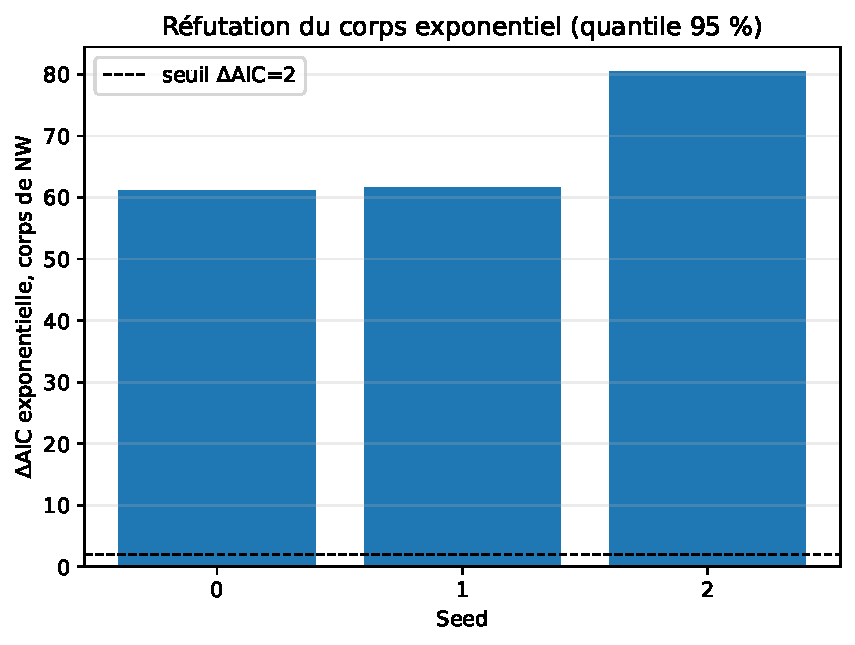
\includegraphics[width=0.66\textwidth]{figures/body_exponential_delta_aic.pdf}
\caption{L'exponentielle est très au-delà du seuil usuel $\Delta$AIC $\leq 2$
sur les trois seeds de baseline.}
\end{figure}

\section{La queue de Pareto est-elle stable ?}

Pas au sens requis. Les seeds 0 et 1 ont des exposants de $NW$ assez stables,
autour de 2,8--2,9. Le seed 2 passe de 2,54 à 3,05 avec $x_{\min}$ de 324 à
857. Surtout, une log-normale correctement normalisée sur $x \geq x_{\min}$ a
une vraisemblance supérieure dans toutes les fenêtres et variables. La Pareto
n'est donc pas identifiée face à la log-normale.

\begin{figure}[ht]
\centering
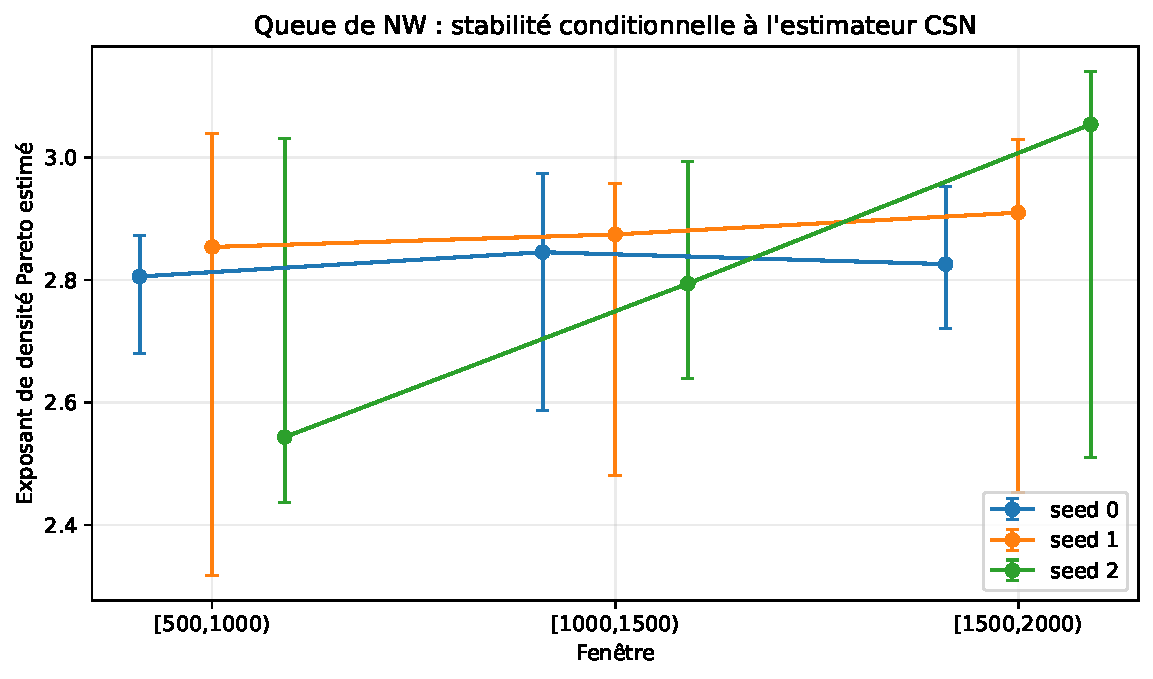
\includegraphics[width=0.86\textwidth]{figures/tail_alpha_windows.pdf}
\caption{Estimations CSN et intervalles bootstrap par blocs, par seed et
fenêtre temporelle.}
\end{figure}

\section{Les classes sont-elles dynamiques ou démographiques ?}

Dynamiques au sens de mobilité de rang et de mortalité. Ce résultat est le
plus solide de l'étude. Il ne prouve toutefois pas l'existence de classes
sociales au sens économique : le modèle représente surtout des états de
bilan sous sélection démographique.

\section{La population est-elle bornée endogènement ?}

La baseline produit un quasi-plateau sans capacité artificielle, mais le
bornage asymptotique n'est pas démontré : les pentes sur $[1000,2000]$
restent positives. Le résultat n'est pas robuste sur la grille. À
$\sigma = 0{,}15$, certaines marges de naissance donnent zéro à cinq
faillites et une croissance presque linéaire.

\begin{figure}[ht]
\centering
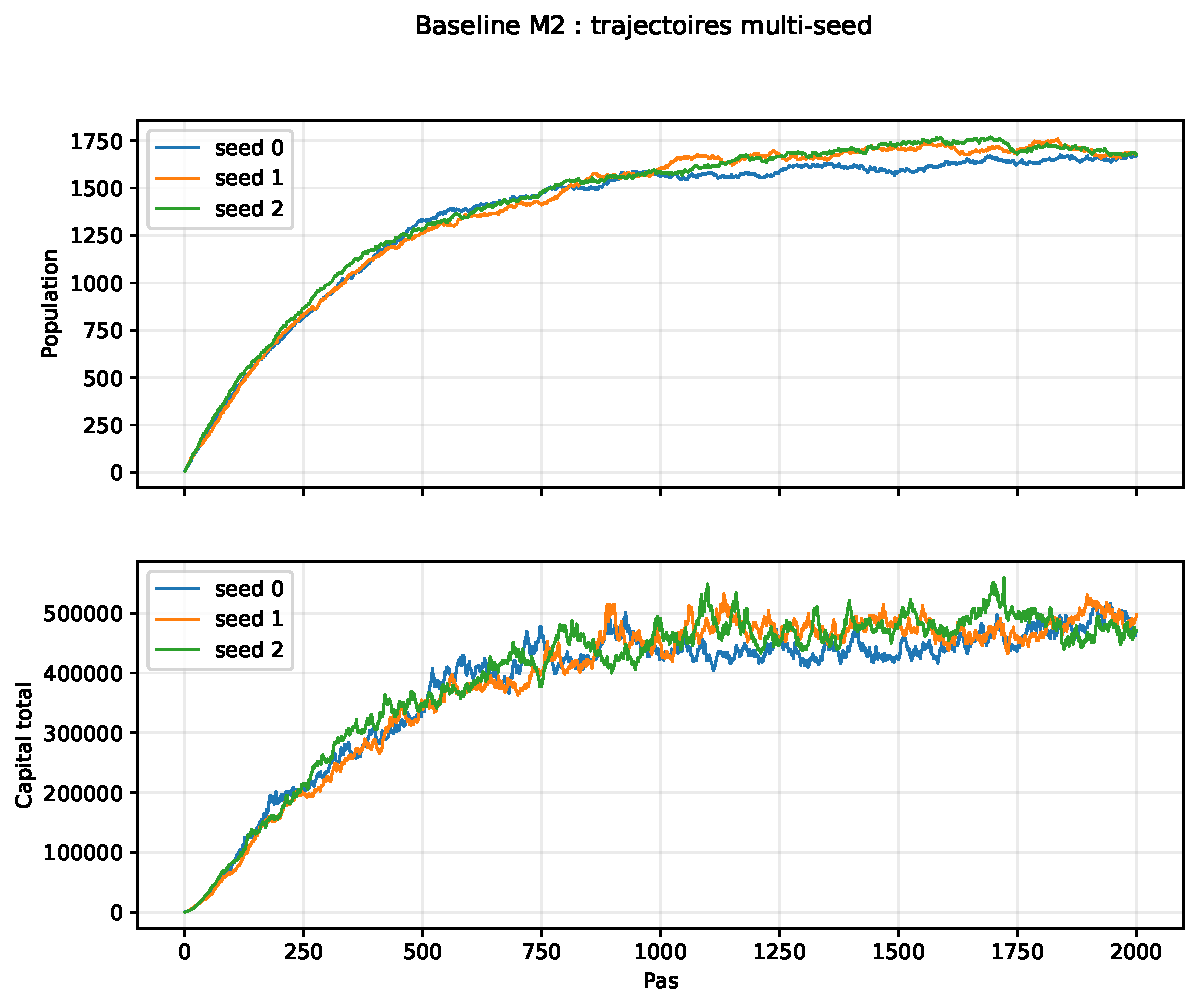
\includegraphics[width=0.9\textwidth]{figures/baseline_multiseed.pdf}
\caption{Trajectoires de population sur trois seeds : reproductibles, en
ralentissement, mais avec une dérive résiduelle positive.}
\end{figure}

\section{Le modèle est-il robuste sans réglage fin ?}

Non. La forme du corps échoue partout, et l'existence du régime
démographique dépend fortement de $\sigma$ et $\varepsilon_0/w_0$. $k$ a
moins d'effet, mais aucune phase SOC robuste n'est identifiée.

\begin{figure}[ht]
\centering
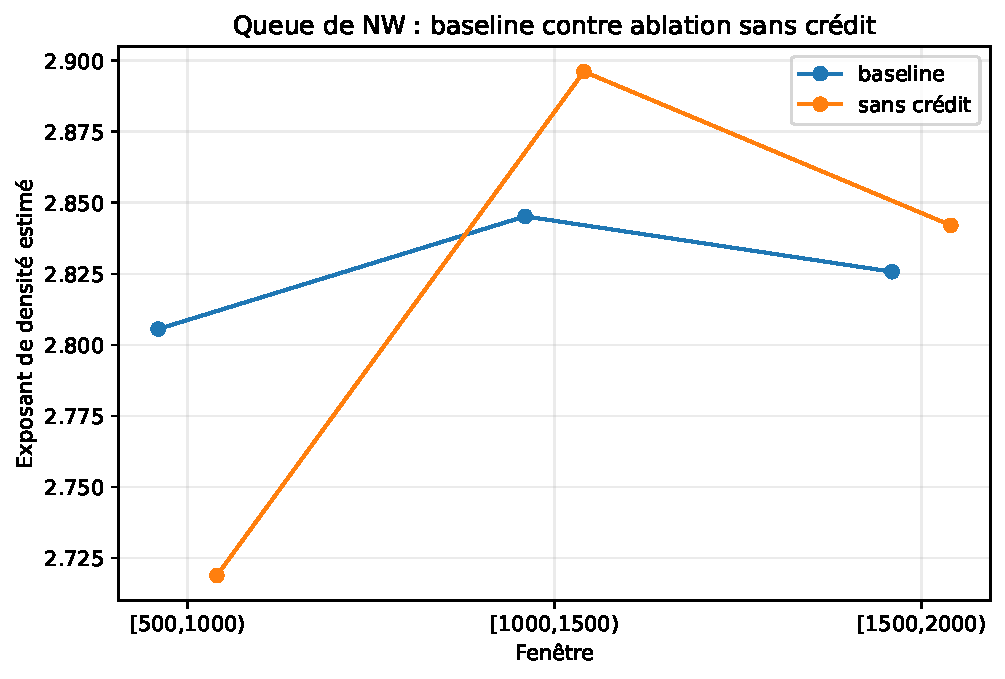
\includegraphics[width=0.8\textwidth]{figures/baseline_vs_no_credit_tail.pdf}
\caption{La suppression complète du crédit ne supprime pas les exposants de
queue observés : le crédit n'est pas la cause nécessaire de la signature.}
\end{figure}

\section{Quelles expériences faut-il lancer ensuite ?}

\begin{enumerate}[leftmargin=1.6em]
  \item Prolonger baseline et ablation sans crédit à 4000--10000 pas.
  \item Répéter sur trois seeds les frontières de grille, surtout
    $\sigma = 0{,}15$ et $\sigma = 0{,}35$.
  \item Tester l'invariance temporelle avec $\delta/2$ et un horizon doublé,
    puis l'extensivité en $\lambda$.
  \item Construire des avalanches causales séparant forçage et relaxation ;
    les lots actuels par pas mélangent plusieurs déclencheurs.
  \item Inclure les morts dans l'estimation des incréments $A_0$, $B_0$.
  \item Comparer Pareto, log-normale et processus de Kesten en prédiction
    hors échantillon.
  \item Tester liquidation simultanée, moyenne de taux et règle de transfert
    comme variantes nommées d'un modèle ultérieur, sans recalibrer M2 après
    coup.
\end{enumerate}

\section{Livrables}

\begin{itemize}[leftmargin=1.4em]
  \item Code : \texttt{src/m2/}
  \item Tests : \texttt{tests/}
  \item Expériences : \texttt{experiments/m2/}
  \item Runs et artefacts : \texttt{outputs/}
  \item Inventaire : \texttt{reports/00\_inventory.md}
  \item Lecture critique : \texttt{reports/01\_critical\_reading/main.pdf}
  \item Spécification : \texttt{reports/02\_technical\_spec/main.pdf}
  \item Implémentation : \texttt{reports/03\_implementation\_report/main.pdf}
  \item Validation : \texttt{reports/04\_validation\_report/main.pdf}
  \item Résultats négatifs : \texttt{reports/05\_negative\_results/main.pdf}
  \item Journal : \texttt{reports/research\_log.md}
\end{itemize}

Commande de test :

\small
\begin{verbatim}
cd /home/anatole/jupyter/modeles/anciens_modeles/m2_codex
PYTHONPATH=src /home/anatole/jupyter/.venv/bin/python3 -m unittest discover -s tests -v
\end{verbatim}
\normalsize

\end{document}
